\documentclass{article}

\usepackage[margin=1in]{geometry}
\usepackage{graphicx}
\usepackage{float}
\usepackage{subfigure}
\usepackage{enumerate}
\usepackage{siunitx}

\title{EE 445L Lab 11 Report: Picocopter}
\author{Reece Stevens and Alex Gerome \\ rgs835, apg744}
\date{December 2, 2016}

\begin{document}
\maketitle

\section{Objectives}
Below is the requirements document for picocopter, a very tiny quadcopter.

\section{Overview}

\subsection{Objectives}
\textit{Why are we doing this project? What is the purpose? }\\ \\
The purpose of this project is to design an embedded system from the ground up. This will give students experience on every part of the design cycle. It also gives students an opportunity to design and print their own PCB, and design their own software system. Our specific project is planned to be a self hovering/stablizing quadcopter.

\subsection{Roles and Responsibilities}
\textit{Who will do what? Who are the clients?}\\ \\
The engineers are Reece Stevens and Alex Gerome, and the TA is the client. The group has modified the provided requirements document to clarify exactly what we plan to build. Our current plans are to work on each part of the lab in tandem.

\subsection{Interactions with Existing Systems}
\textit{How will it fit in?}\\ \\
The system will use the TM4C123 chip, and a specially printed PCB to handle our needs.


\section{Function Description}

\subsection{Functionality}
\textit{What will the system do precisely?}\\ \\
The system will be a quadcopter. It will be designed to hover and stablize itself in a 3D space. Once turned on, it will levitate to a certain height, and then maintain that position until turned off.

\subsection{Performance}
\textit{Define the measures and describe how they will be determined.}\\ \\
All software must be clear and concise. The PCB and hardware must also be laid out in a manner that makes sense, and minimizes PCB area; this is to reduce the footprint of the system. The system's success will be measured by the stability of the system while hovering, and it's ability to regain stability when disrupted.


\subsection{Usability}
\textit{Describe the interfaces. Be quantitative if possible.}\\ \\
There will be an on/off switch for the system. Once activated, the system will turn off, and the accelerometer will send data to the TM4C chip. The accelerometer will be used to stablize the quadcopter.

\subsection{Safety}
\textit{Explain any safety requirements and how they will be measured.}\\ \\
Since we are dealing with a flying object, the system will not be run in close quarters, and necessary precaution will be taken when people are nearby.

\section{Deliverables}

\subsection{Reports}
\textit{How will the system be described?}\\ \\
Lab reports for labs 7 and 11 will be written, and necessary source files will be submitted.

\subsection{Outcomes}
\textit{What are the deliverables? How do we know when it is done?}\\ \\
There are three deliverables: preparation, demonstration, and report. The following will be included with Lab 7:
\begin{enumerate}[A)]
\item Objectives: 1-page requirements document
\item Hardware Design: Regular circuit diagram (SCH file), PCB layout and three printouts (top, bottom and combined) 
\item Software Design: Include the requirements document (Preparation a)
\item Measurement Data: Give the estimated current (Procedure d), Give the estimated cost (Procedure e)
\item Analysis and Discussion: (none)\\
\end{enumerate}

And the following are the contents of the lab 11 report:
\begin{enumerate}[A)]
\item Objectives: 2-page requirements document
\item Hardware Design: Detailed circuit diagram of the system (from Lab 7)
\item Software Design: (no software printout in the report) Briefly explain how your software works (1/2 page maximum)
\item Measurement Data: Include data as appropriate for your system. Explain how the data was collected.
\item Analysis and Discussion: (none). The YouTube video is required
\end{enumerate}


\section{Hardware Design}
\begin{figure}[H]
	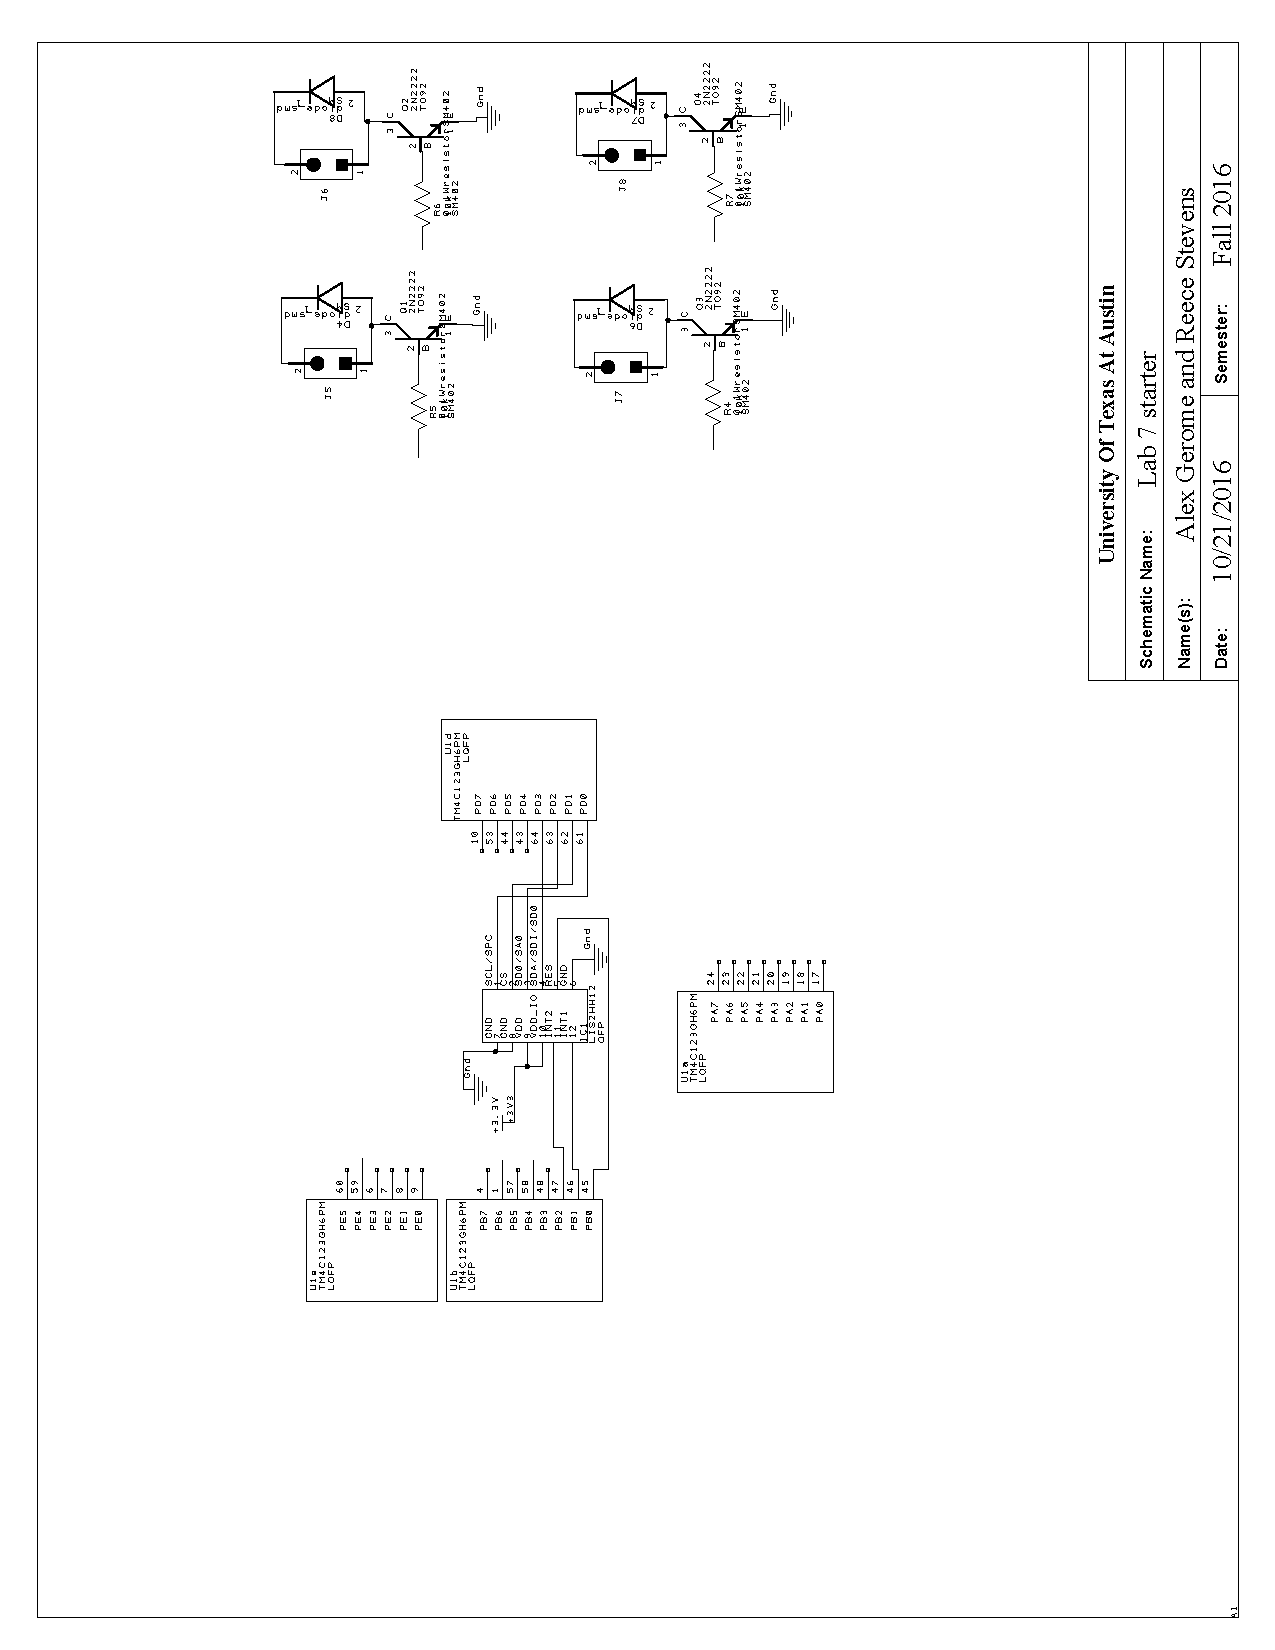
\includegraphics[width=\textwidth]{./CircuitSchematic}
    \caption{Regular circuit diagram.}
\end{figure}

\begin{figure}[H]
	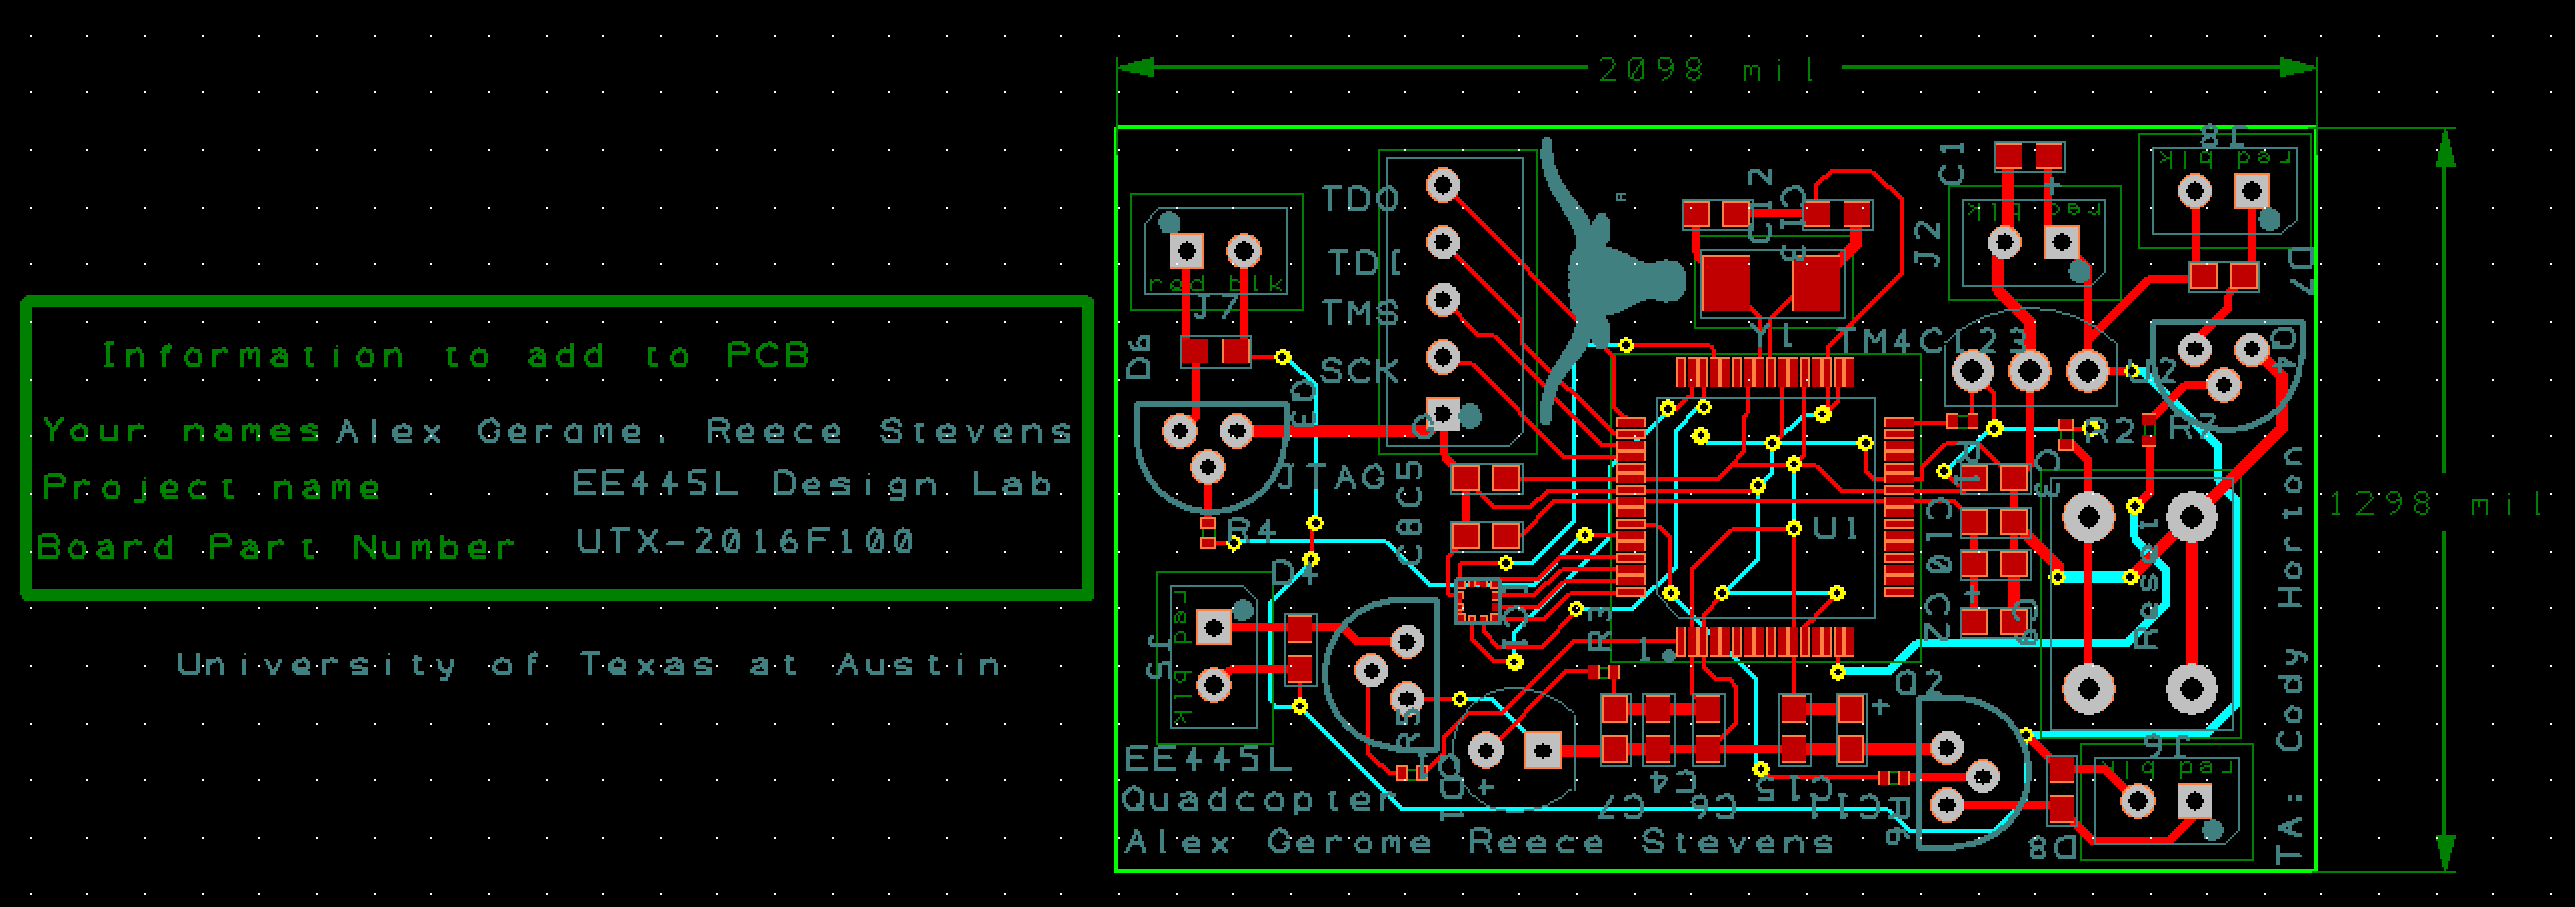
\includegraphics[width=\textwidth]{./PCB_both}
    \caption{Combined PCB Layout}
\end{figure}

\section{Software Design}
% TODO: How the software works

\section{Measurement Data}
% TODO: Measurement data

\section{Analysis and Discussion}
None for this lab.

\end{document}
